The goal of this project is to create an efficient genealogy tree. As input your
program will read a list like the following:

\begin{verbatim}
1 4 5
1 4 5
0 1 6
0 1 7
2 1 3
0 1 2
0 1 3
0 1 4
0 5 3
0 5 6
1 2 1
0 4 4
-1 0 0
\end{verbatim}

Each line represents a relation parent/child between to people, with three items:

\begin{verbatim}
relation id_p1 id_p2
\end{verbatim}

\textit{relation} can be: either 0 [child] or 1 [parent]. \textit{id\_p1}
and \textit{id\_p2} are IDs of the two people involved. Thus for
example: \textit{1 4 5} means that 5 is a parent of 4, while \textit{0 1 6} means
that 6 is a child of 1.

The code should ignore: duplicated relations and relations with wrong number
(i.e. not 0 or 1). At the same time, your code should have for each node a
maximum of 4 parents and 4 children, so we should also skip if we try to add
more than 4 parents or 4 children for a node.

A \textit{relation} of -1 is used to identify the end of the input.

Thus, the relations given above represent a genealogy tree as can be seen in
figure \ref{fig:genealogy-1}. Note that 4 is considered to be a child of itself!
and that the relation ``0 1 7'' has been dropped because node 1 already has 4
children.

\begin{figure}[!htbp]
  \centering
  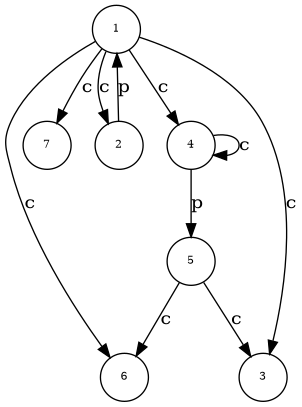
\includegraphics[width=0.3\textwidth]{graphics/projects/gen1.png}
  \label{fig:genealogy-1}
  \caption{Relations graph - 'c' (child); 'p' (parent)}
\end{figure}


Your goal is to create a Binary Search Tree where the nodes will be sorted based
on their ID, but at the same time, each node will include links to its parents
and its children (not the IDs of its children and parents, but pointers to the
appropriate nodes in the tree). Thus, the BST would look like
figure \ref{fig:genealogy-2} (assuming you add nodes to the tree as they appear
in the input file above), with the arrow representing the usual left/right
nodes, but on top of that, you should make sure that each node maintains links
to its children and parents.

\begin{figure}[!htbp]
  \centering
  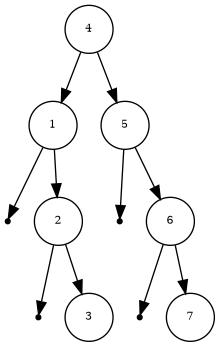
\includegraphics[width=0.2\textwidth]{graphics/projects/gen2.png}
  \label{fig:genealogy-2}
  \caption{BST}
\end{figure}


The graph with all the arrow pointing left/right, with all the children and
parents become messy quite quickly, but we can see an example of how it would
look like in figure \ref{fig:genealogy-3}, which is only a restricted view, with
the relations for nodes 4,1 and 5. We see that the left pointer of 4 points to 1
and the right pointer to 5, thus keeping the structure of the BST as shown above
in figure \ref{fig:genealogy-2}. At the same time, the first child (c1) of node
4 points to itself (node 4), while the first parent (p1) of node 4 points to
node 5, etc. So you can see that what you are supposed to do is just build the
BST tree according to the ID of each person, but then make sure that you link
the children and parents pointers according to the relations in the input file.

\begin{figure}[!htbp]
  \centering
  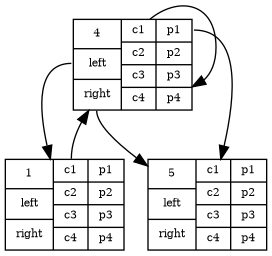
\includegraphics[width=0.4\textwidth]{graphics/projects/gen3.png}
  \label{fig:genealogy-3}
  \caption{BST with full connections, restricted to nodes 4,1 and 5}
\end{figure}

Remember that in Fortran you cannot have an array of pointers, but this is
easily done by having a derived type which only component is a pointer and then
having an array of that new type. To make this easier for you, the type
definitions needed for each of the nodes could be something like:

\begin{verbatim}
  TYPE CPtr
     TYPE(PERSON), POINTER :: ptr
  END type CPtr
  
  TYPE PERSON
     INTEGER :: id
     TYPE(PERSON),POINTER :: left,right
     TYPE(CPtr), DIMENSION(4) :: parents
     TYPE(CPtr), DIMENSION(4) :: children
  END type PERSON
\end{verbatim}

When you write the code, make sure that it does two things:

\begin{enumerate}
\item Create the tree, printing when a new node is created, and giving warnings when:
 there is no space to hold more relations in a node; a relation has already been
 created; the relation type is wrong
\item Print the tree, following the way we printed a BST tree in the lectures,
 from the smallest ID to the biggest ID, printing for each node its parents and children. 
\end{enumerate}

Remember that the project is not all or nothing, and your mark will depend on
how far you get, but you can submit partial code, non-working code (if possible
with comments) and even a text explanation of things that you tried to do but
don't work, etc.

Try to start simple and build up the code when you are sure the previous step
works. For example, try first to generate the BST tree for the people
ID and verify that it is well formed, but ignoring the relations. Once that
is properly done you can start adding relations but ignoring the warnings
(thus, assuming that the input file will never have, for example, repeated relations),
and at the end adding the code to check the warning situations. Keep copies of
the code as you get partial solutions, so that you can at least submit something
that works in the case that the next steps become difficult and you cannot solve
them. Also, remember that this is an INDIVIDUAL project. You can discuss generic
ideas, but the final code has to be yours. 


Lastly, as an example of what your code should produce when giving the above
input file, it could look like this:

\begin{verbatim}
[angelv]$ ./gen < gen.in
 
 -----------------------
 CREATING GENEALOGY TREE
 -----------------------
 creating new node           4
 creating new node           5
 ... WARNING: relation           1           4           5 already entered, skipping
 creating new node           1
 creating new node           6
 creating new node           7
 creating new node           3
 ... WARNING: wrong relation value           2 , skipping
 creating new node           2
 ... WARNING: no empty places for           0           1           4 , skipping
 
 -----------------------
 PRINTING GENEALOGY TREE
 -----------------------
 
 ------------ node            1 --------------
 PARENTS
 CHILDREN
           6
           7
           2
           3
 
 ------------ node            2 --------------
 PARENTS
           1
 CHILDREN
 
 ------------ node            3 --------------
 PARENTS
 CHILDREN
 
 ------------ node            4 --------------
 PARENTS
           5
 CHILDREN
           4
 
 ------------ node            5 --------------
 PARENTS
 CHILDREN
           3
           6
 
 ------------ node            6 --------------
 PARENTS
 CHILDREN
 
 ------------ node            7 --------------
 PARENTS
 CHILDREN

[angelv]$
\end{verbatim} 
